% exercise sheet with header on every page for math or close subjects
\documentclass[12pt]{article}
\usepackage[utf8]{inputenc} 
\usepackage{latexsym} 
\usepackage{multicol}
\usepackage{fancyhdr}
\usepackage{amsfonts} 
\usepackage{amsmath}
\usepackage{amssymb}
\usepackage{enumerate}
\usepackage{listings}
\usepackage{graphicx}

% Shortcuts for bb, frak and cal letters
\newcommand{\E}{\mathbb{E}}
\newcommand{\V}{\mathbb{V}}
\renewcommand{\P}{\mathbb{P}}
\newcommand{\N}{\mathbb{N}}
\newcommand{\R}{\mathbb{R}}
\newcommand{\C}{\mathbb{C}}
\newcommand{\Z}{\mathbb{Z}}
\newcommand{\Pfrak}{\mathfrak{P}}
\newcommand{\Pfrac}{\mathfrak{P}}
\newcommand{\Bfrac}{\mathfrak{P}}
\newcommand{\Bfrak}{\mathfrak{B}}
\newcommand{\Fcal}{\mathcal{F}}
\newcommand{\Ycal}{\mathcal{Y}}
\newcommand{\Bcal}{\mathcal{B}}
\newcommand{\Acal}{\mathcal{A}}


% Formatierung
\topmargin -2cm 
\textheight 24cm
\textwidth 16.0 cm 
\oddsidemargin -0.1cm

\setlength{\parindent}{0pt}  % !!!!!!! Hier werden leerzeilen erlaubt ohne dass Latex automatisch einrueckt! !!!!!!! %


\graphicspath{ {images/} }


\begin{document}

% Titel
%\title{\textsc{Hacking}\\ \textsc{Abgabe 0}\\{ \normalsize Gruppe X \hfill Daniel Schäfer (2549458)\\ \hfill Anderer}}
%\maketitle  

% alternativer Titel
\noindent
{\Large \textbf{High-level Computer Vision}} \hfill \textbf{26.05.2016}\\
{\Large \textbf{Exercise 3}} 
\raggedleft \hfill Guillermo Reyes (2556018)\\
\hfill Daniel Schaefer (2549458)\\
\hfill Marc Tonsen (2537359)\\
\hfill Dominik Weber (2548553)\\

\pagenumbering{gobble}
\raggedright


\section*{Code Annotations}
we ''disable'' L2 normalization by changing the part to
\begin{verbatim}
  % disabled L2 normalization for overlapping blocks 
  % Four cells are combined into one block
  % One cell maximumly contributes to 4 blocks
  %
  for by = 1:(PARAMS.num_cells_height-1)
      for bx = 1:(PARAMS.num_cells_width-1)
          %
          % add the L2 block-normalization step here
          %
          % ...
          v = [CELLS{by, bx}; CELLS{by, bx+1}; CELLS{by+1, bx}; CELLS{by+1, bx+1}];
          v = v(:);
          % v = v ./ (sum(v .^ 2) + e);
          % ...
          DESC = [DESC; v];
      end
  end

\end{verbatim}




\section*{Question 1: Support Vector Machines}

\begin{enumerate}[a)]
	\setcounter{enumi}{1}
	\item 	
        \textbf{Modify the last two parameters of} \verb!get\_train\_dataset\_2d.m! \textbf{in order to make the classification problem linearly non-separable. Run your visualization for different values of parameter C and comment on its role in the SVM classification algorithm.}\\
        
        	\begin{figure}[h]			
        		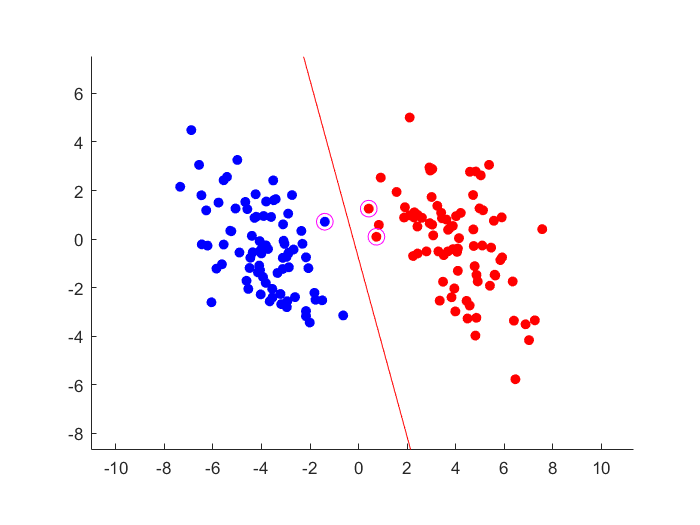
\includegraphics[width=0.5\textwidth]{1b_separable}
        		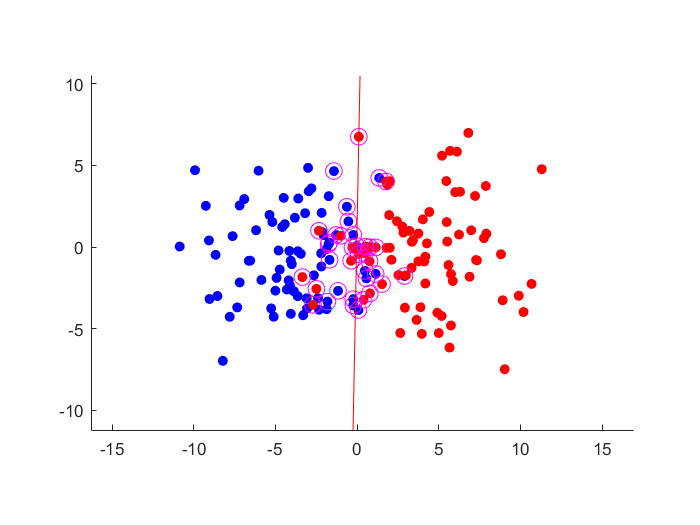
\includegraphics[width=0.5\textwidth]{1b_non-separable}
        		\caption{\textit{Left}: SVM for linearly separable data with default parameters. $ \sigma_1=1.5, \sigma_2=5 $. \textit{Right}: SVM for linearly non-separable data. The same parameters are used to generate the data except that $ \sigma_1=10 $ and $\sigma_2=10 $ and $C=100$ }
        	\end{figure}
        In Figure 1 we can see on the left, the linearly separable data of two distributions. The best fit for a separating hyperplane results in a margin of 1.88 and 3 support vectors. By making the the sigmas of the distributions large enough, we are effectively making the data more spread, and thus, the two distributions overlap. the result is the image on Figure 1, right.  By generating the data with $\sigma_1=10 $ and $\sigma_2=10 $ the the two distributions share a common region in space and are therefore no longer separable. How ever by using a soft margin SVM we can still fit the hyperplane that best "splits" the data i.e. the one with largest margin. In this case we can get a margin of about 3.45 with 38 support vectors.
        
        
           	\begin{figure}[h]			
          		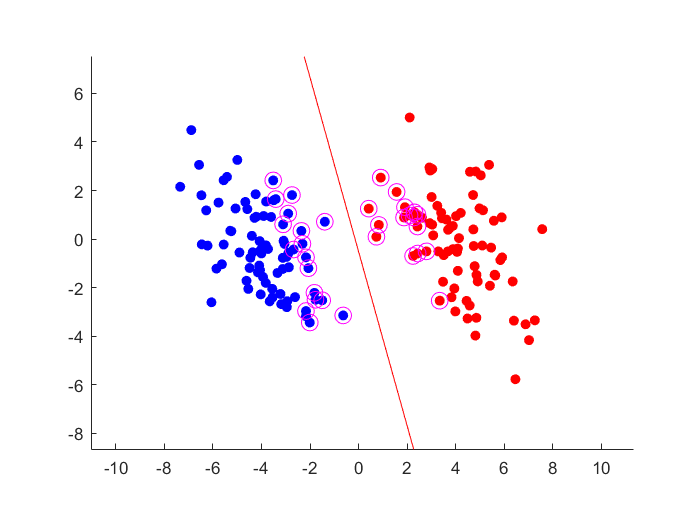
\includegraphics[width=0.5\textwidth]{1b_separableC005}
           		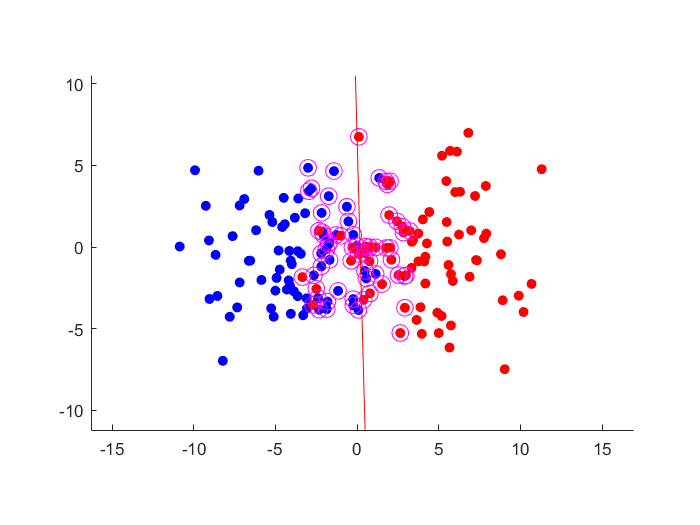
\includegraphics[width=0.5\textwidth]{1b_non-separableC005}
          		\caption{\textit{Left}: SVM for linearly separable data with default parameters. $ \sigma_1=1.5, \sigma_2=5, C = .005$ The margin is 5.48 and there are 34 support vectors. \textit{Right}: SVM for linearly non-separable data. The same parameters are used to generate the data except that $ \sigma_1=10, \sigma_2=10, C=.005 $. Here the margin is around 6.1 and there are 66 support vectors }
           	\end{figure}
        
		The parameter C is used in the minimized loss function to tune the importance of the sum of $\xi$'s. A high value for C would put a lot of importance on them and would therefore force them to take very small values. Therefore, the higher the value of C is, the closer the performance comes to that of a hard-margin SVM. If C has a small value this would soften the margin and would also allow support vectors inside the margin, even when the data is linearly separable. In Figure 2, left we can see and example if this: the data was generated by the same parameters as in Figure 1, but the selected C is .005, which allows the margin to grow to 5.48 and the use of 34 support vectors (against 3 used before). In Figure 2, right we also see how setting the parameter C to a lower value allows the margin to be softer. In conclusion C influences how soft the margin of the SVM is for both: linearly separable and non-linearly separable data.
\end{enumerate}

\newpage
\section*{Question 3: Performance Evaluation}
\begin{enumerate}[a)]
	\setcounter{enumi}{3}
	

	\item
        \textbf{Write a summary of your observations and submit it along with the corresponding RPC curves}\\
        
        \begin{figure}[h]			
        	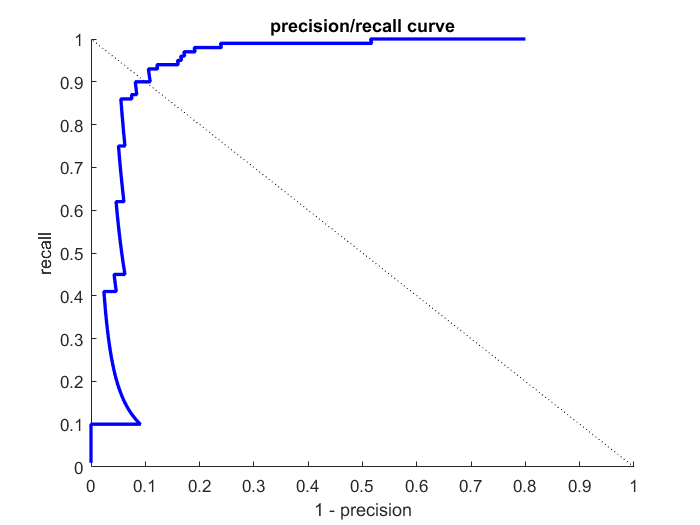
\includegraphics[width=0.5\textwidth]{rpc_norm8}
        	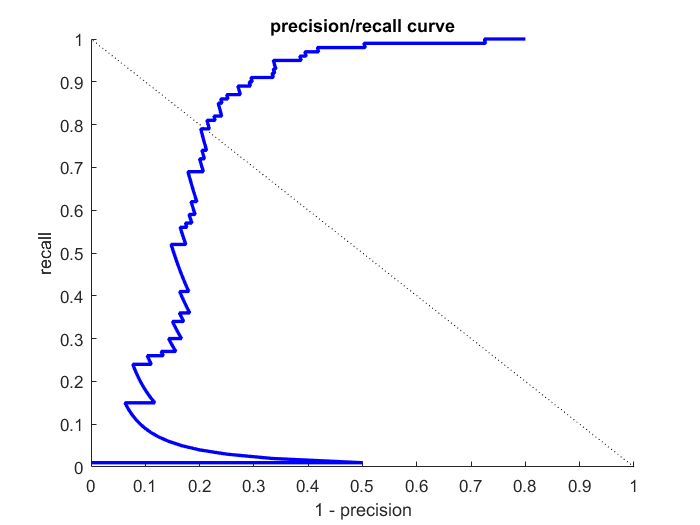
\includegraphics[width=0.5\textwidth]{rpc_not_norm8}
        	\caption{Comparison of RPC curves with and without normalization. \textit{Left}: RPC curve with normalization step and cell size of 8 pixels. \textit{Right}: Same kind of curve without normalization step.}
        \end{figure}
        
        The overall recognition rate corresponding the the RPC curve on Figure 3 to the right is of 93.4\%. Compared against its neighbor on the right which is of 89.2\%, it is slightly superior. It is interesting to note that the number of false positives detected (31) is clearly larger in both cases than the overall false negatives detected (2) , and both increase even more when not performing the normalization step (49 and 5 respectively).
        
        \begin{figure}[h]			
        	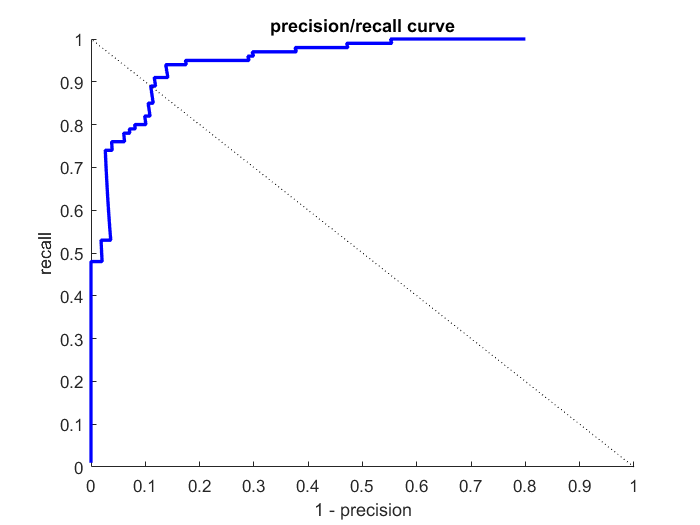
\includegraphics[width=0.5\textwidth]{rpc_norm16}
        	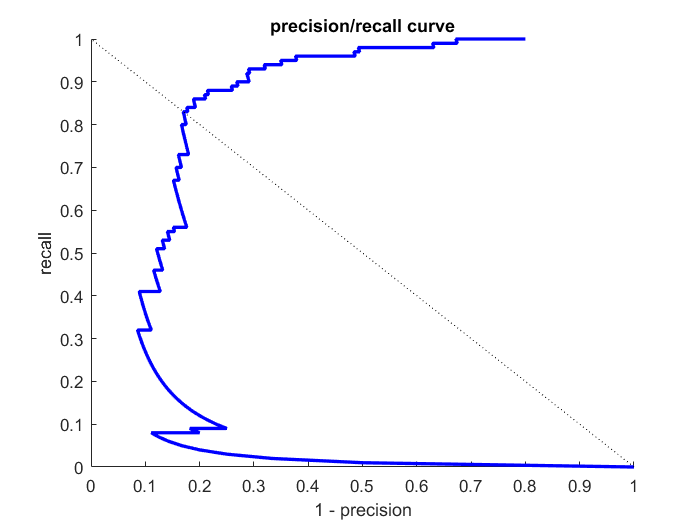
\includegraphics[width=0.5\textwidth]{rpc_not_norm16}
        	\caption{Comparison of RPC curves with different cell sizes. \textit{Left}: RPC curve with normalization step and cell size of 16 pixels. \textit{Right}: RPC curve without normalization step and cell size 16. }
        \end{figure}
        
        When looking at the RPC curves for cell sizes of 16 pixels (Figure 4) one surprising this to see is not the same kind of behavior as for cells of 8 pixels (Figure 3): When not doing the normalization step, the overall recognition rate actually increases slightly (from 86\% to 87.4\%). One might argue that this improvement is minor and merely a coincidence, but it is not to be ignored. Here we also note that, regardless, both with and without the normalization step, the recognition rate is still inferior to the SVMs that use a a cell size of 8. Another important observation is that here, again, the amount of false positives is clearly larger than the number of false negatives (68 vs 2  when doing the normalization step and 59 vs 4 when not doing it). In fact, increasing the cell size seems to only harm false positives, while actually benefiting false negatives in the case of not doing the normalization step.\\
        
    %TODO Explain why these observations happen


		\textbf{Our Explanations:}\\    
		 The fact that Cell size 16 has a little bit better result using no L2 normalization can only be coincidence depending on the training and test samples, especially because the difference is so minor. Cell size 8 performs overall superior to Cell size 16 because the normalization on Cell Size 8 makes local contrasts much more visible and stronger compared to Cell size 16.
	    
	    We also noticed that the amount of false positives was much larger than the amount of false negatives. We must first consider that the number of negative images is 4 times larger than the positive one, so we would expect about 4 times less false positives if we took also 4 times less negative images. Even then we would still have more false positives, but we think the difference is only random and is by no means generalizable and lies only in the data taken for this exercise. 
    
    %TODO Conclusions
         

	\item 
        \textbf{How could you use the system to solve the detection problem in which you are given an image of arbitrary size and the task is to find the position of the people in it?}\\
        We could train the system a few times to work on images of different scale (i.e. train a separate system per scale). Then we could run those systems on the input image of arbitrary size in a sliding window fashion: For each scale pick uniformly spread patches of that size from the image and run the classifier on them. If the content of a patch is classified as an object of interest, we can return the bounding box of that patch as a detection result for that kind of object. One should be careful not to report the same object multiple times because it was recognized in multiple patches. Comparing the spacial relation of the bounding boxes can help to find the tightest bounding box out of all candidates. \\
        This way we can recognize and localize objects in the input image with only our classification system. However the accuracy of the localization is limited by the smallest scale for which we have a classifier (i.e. the smallest possible bounding box corresponds to the size of the smallest scale) and objects in the image that are bigger then the size of the largest scale might not be found.\\
        Assuming we don't care about the time our programm takes to detect the human, we have the possibility to iterate from really tiny patch sizes to very big patch sizes, and move the patches only 1 pixel for every iteration of this patch-size. This way we can return the smallest possible patch we found, which contained a human according to our algorithm without having to iteratate over all possible patch-sizes and all possible patch placements. It's obvious that this naive approach still has extremely terrible running time. It's all about finding a balance here depending on how precise you want the detection to be.

\end{enumerate}


\end{document}
